

% Template PNSAC newsletter
% Language: Latex


\title{Project North Star Trip to  426 Squadron}
\author{Bill Tate}

\maketitle

Friday June 14th dawned bright and clear for our visit to 426 Squadron
at 8 Wing Royal Canadian Air Force Station Trenton.

\begin{figure}[htbp]
   \vspace{2em}
   \centering
   %name of the graphic, without the path AND in EPS format:
   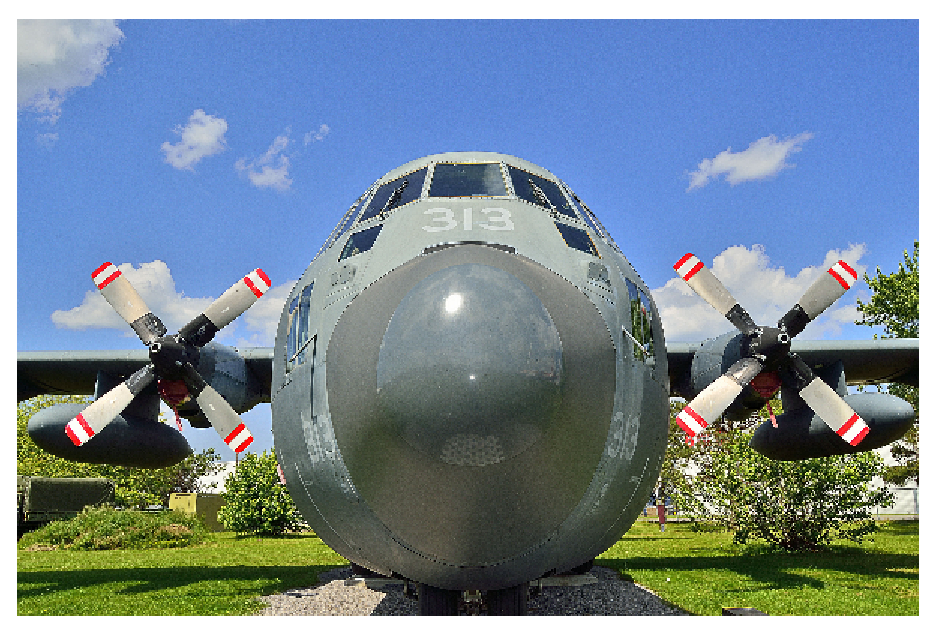
\includegraphics[scale=0.5]{trenton2013-herc.eps}
   %caption of the figure 
   \caption*{\small \em National Air Force Museum -- Hercules.}
   %label of the figure, which has to correspond to \ref{}:
   \label{fig:herc}
\end{figure}

Once again scheduling allowed us to have Jean Pierre as our driver
which meant JP had as much fun as we did. We departed right on time at
07:00 with Richard Lodge giving everyone on board a welcome and a
brief explanation of the day's events.

With the kind assistance of Garry and Jim, all on board were offered
our normal complimentary coffee and donuts to help kick start the
early day. Following a brief stop in Mallorytown on the 401 we
proceeded for what we thought would be an on-time arrival at 426
Squadron but a freight train had other plans for us. After skillful
driving by JP we arrived only 20 minutes late at the Sedley
S. Blanchard Air Mobility Training Center which is the home of 426
Squadron.

Our group was warmly greeted by Lieutenant Colonel Perrault the
Commanding Officer of 426 Squadron who gave us a briefing on what
responsibilities 426 Squadron has in its training role .

After our welcome we were split into groups to start our planned tours
of this very modern high tech facility. One of the many highlights of
the tour was the Fuselage Trainer, a full size fuselage from an old
airframe which is used for training load masters. The Fuselage Trainer
can be integrated with the Tactical Flight Training Device, a
simulator that has full motion with a wrap around visual system. In a
training scenario the Fuselage Trainer can be integrated with the
simulator to offer real time integrated training for both crews. I was
impressed with the new capabilities of the wrap around visual system
which is superior to the older systems that I trained on. While we all
had a chance to hand fly the simulator I was impressed with how
advanced the simulator visual display is, in which you can pick out
the difference of a deciduous tree to a coniferous tree. Another
upgrade is the Heads Up Display or the HUD in which you look through a
screen in front of the cockpit window which has all the flight
instruments projected onto a small screen. The will allow a pilot the
enhanced situational awareness of looking outside the aircraft and
still have the flight instruments for guidance.

Another training aid was the Integrated Procedures Trainer which
allows maintenance and flight crews to work through issues with system
failures. The other part of this was another full scale fuselage with
partial wing where maintenance can be done on a full scale engine with
propeller as well as part of the wing and fuselage.

The other training module was the Night Vision Integrated Simulator
where observers train in tandem with pilots on detection of missiles ,
anti aircraft artillery aka "Triple A" using the latest in restricted
military use only night vision goggles which cost the price of a mid
sized car.

The tour was highly organized and we were all impressed with high
degree of enthusiastic professionalism displayed by all members of 426
Squadron.

After the visit to 426 Squadron we went to the Yukon Galley for a
light lunch before proceeding to the National Air Force Museum for a
tour of the restoration shops, their displays indoors and outdoors.

The day concluded with dinner at Tomasso's Italian Grill before we
drove back to Ottawa to end the day.

\end{multicols}

\begin{figure*}[ht!]
   \vspace{2em}
   \centering
   %name of the graphic, without the path AND in EPS format:
   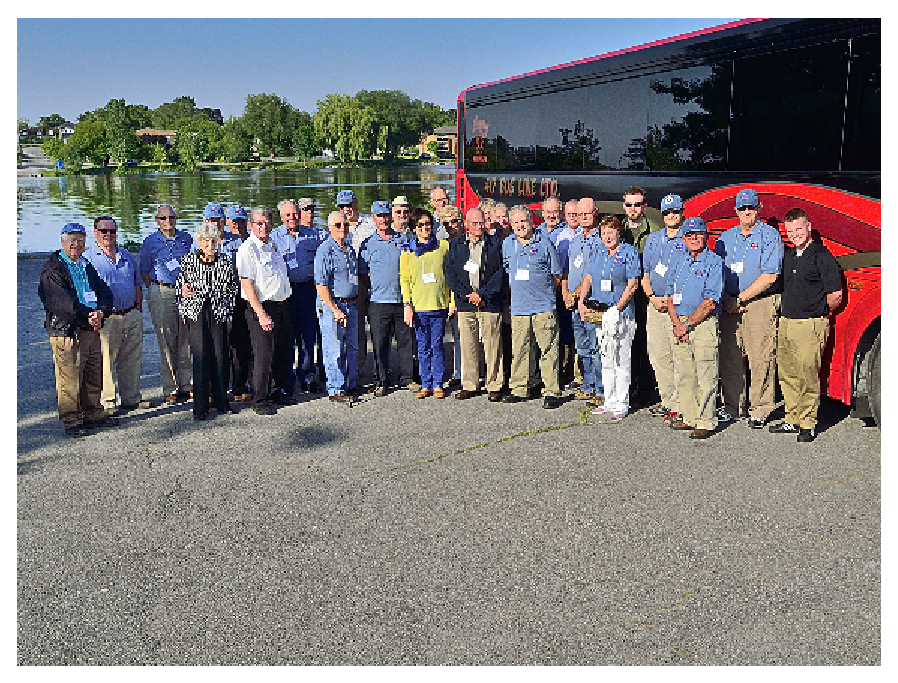
\includegraphics[scale=0.75]{trenton2013_group.eps}
   %caption of the figure 
   \caption*{\small \em After Tomasso's -- ready for the drive home.}
   %label of the figure, which has to correspond to \ref{}:
   \label{fig:rollsroyce}
\end{figure*}

\begin{multicols}{2}


\begin{footnotesize}
    \raggedleft PNSAC\\
\end{footnotesize}

%%% Local Variables: 
%%% mode: latex
%%% TeX-master: main_document.tex
%%% End: 
